\section*{Acknowledgment}
I would like to thank Dr. Raphael Berger for giving me the opportunity to work on this interesting topic, for the introduction to the topic and all the helpful discussions. I also would like to thank Dr. Stuard for the discussions \\
All staff of the chair of inorganic chemistry are acknowledged for the very good working  environment and supporting this work. \\
The chair of theoretical chemistry is acknowledged for providing the computer resources for this work. 
\newpage



\section{Introduction}
Gas phase Electron Defraction  (GED) is a state of the art method for determining molecular structures in gas phase. Even 60 ( CHECK!) years after its invention, analysis of the experimental data is not trivial or automated as it is in X-Ray defraction. An example for these experimental data is visualisded in Figure~\ref{example} (p. \pageref{exaple}). To determine the limits or angle for the data reduction human intuition is still required. The aim of the written program is to provide an convenient way to graphically determine all parameters (limits, angle etc.) for the data reduction. For convenience, a bash-script is written out, that directly does the data reduction with PIMAG (REF!). Also some minor changes on the PIMAG program were made for compatibility reasons. \\
The program runs on all Unix, Linux and Mac OS X systems( Windows support should be easy to implement). \\
This documentation will first explain the graphical user interface of \textit{GED ready} and the workflow (Chapter \ref{interface}. In Chapter~\ref{tech} the technical details of the program itself will be discussed in detail. 
 
\begin{figure}
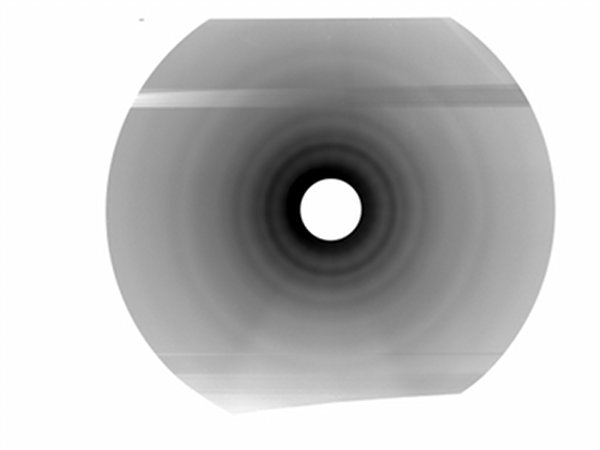
\includegraphics[width=12cm]{example}
\caption{An example of the raw data from the GED experiment.}
\label{example} 
\end{figure} 


 